\section{下界的构造}
\label{sec:dual-lower-bound}

对一般的约束问题，怎样写出一个不依赖未知最优点的下界？全章讨论的问题是
\begin{equation}
 \begin{aligned}
 \min_{\bm{x}\in\bm{D}}\quad & f(\bm{x})\\
 \text{s.t.}\quad & g_i(\bm{x})\leq0,\quad i=1,\ldots,m,\\
 & h_j(\bm{x})=0,\quad j=1,\ldots,p.
 \end{aligned}
 \label{eq:dual-primal}
\end{equation}
这里$\bm{D}\subseteq\mathbb{R}^n$是规定的定义域，$f,g_i,h_j$在其上都取有限值。没有特别说明时$\bm{D}=\mathbb{R}^n$；有些问题只在一部分点上有定义，或者我们有意把一些简单约束（例如$\bm{x}\geq\bm{0}$）留在$\bm{D}$里。

式~\eqref{eq:dual-primal}称为原始问题，它的最优值记为$f^\star$，是可行点上目标值的下确界。没有可行点时规定$f^\star=+\infty$。我们不假设最小点存在，也不假设问题是凸的，这两点在后面都很重要。

第~\ref{chap:constrained-optimality}章为这个问题定义了Lagrange函数，给每条不等式配乘子$\lambda_i$，每条等式配乘子$\nu_j$：
\begin{equation}
 \mathcal{L}(\bm{x},\bm{\lambda},\bm{\nu})=f(\bm{x})+\sum_{i=1}^m\lambda_ig_i(\bm{x})+\sum_{j=1}^p\nu_jh_j(\bm{x}).
 \label{eq:dual-lagrangian}
\end{equation}
那里用它写出候选点上的驻定条件，这里换一个用法：把它当成原目标的一个替身。

\paragraph{用线性价格代替无穷的墙}
约束可以看成目标里的一堵墙。令$\iota_{\leq0}(u)$在$u\leq0$时为$0$，在$u>0$时为$+\infty$，则不等式约束等价于在目标上加$\iota_{\leq0}(g_i(\bm{x}))$。这个函数太硬，无法与目标一起处理。

换成一条斜率$\lambda\geq0$的直线$\lambda u$。图~\ref{fig:dual-wall-price}(a)显示，不论$\lambda$取多少，直线都在墙的下方：$u\leq0$时$\lambda u\leq0$，$u>0$时墙是$+\infty$。用直线替换墙，得到的函数不会超过原来带墙的目标。

这正是价格的想法。约束超支一单位就付$\lambda$的罚款，有结余就按同样的价格退款，违反约束不再被禁止，只是要付钱。等式约束的乘子$\nu_j$没有符号限制，因为$h_j=0$时无论乘什么数，这一项都为零。这个类比只帮助记住不等式的方向，并不表示真的存在这样的市场。

下面用一个能画出来的例子走一遍，全章称它为\emph{一元例}：
\begin{equation}
 \min_{x\in\mathbb{R}}\ \frac12(x-2)^2\quad\text{s.t.}\quad x-1\leq0.
 \label{eq:dual-oned}
\end{equation}
无约束最小点$x=2$不可行，所以解在边界$x^\star=1$上，最优值$f^\star=1/2$。

取$\lambda=1/2$，Lagrange函数是
\[
 \mathcal{L}(x,\tfrac12)=\frac12(x-2)^2+\frac12(x-1).
\]
在可行点$x\leq1$上，第二项不大于零，所以$\mathcal{L}(x,\frac12)\leq f(x)$。图~\ref{fig:dual-wall-price}(b)中，紫色曲线在阴影区都位于蓝色曲线下方，并且全部经过$(1,\frac12)$，因为那里约束的值恰好为零。

对$x$求最小，驻点满足$x-2+\frac12=0$，即$x=\frac32$，最小值是
\[
 \mathcal{L}(\tfrac32,\tfrac12)=\frac18+\frac14=\frac38.
\]
这个最小点并不可行，这没有关系。它是$\mathcal{L}$在整条数轴上的最小值，当然不超过$\mathcal{L}$在可行点上的值，而后者又不超过$f$。于是我们没有用到$x^\star$，就知道$f^\star\geq3/8$。

\begin{BookInlineFigure}
 \centering
 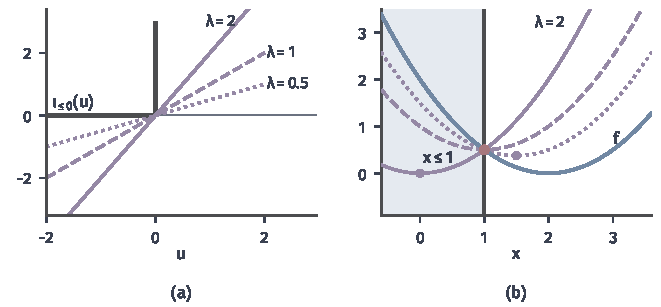
\includegraphics[width=112mm]{figures/05-optimization/06-constrained-optimization/matplotlib/dual-wall-price/figure.pdf}
 \caption{用线性价格代替硬约束。(a)~深灰粗线是硬约束$\iota_{\leq0}(u)$，紫线是$\lambda u$，点线、虚线、实线分别对应$\lambda=0.5,1,2$，都在粗线下方。(b)~一元例~\eqref{eq:dual-oned}：蓝线是目标$f$，浅蓝区域是可行集$x\leq1$，紫线是$\mathcal{L}(\cdot,\lambda)$，线型含义同(a)；紫点是各自的最小点，红点是原始最优点。}
 \label{fig:dual-wall-price}
\end{BookInlineFigure}

这段推理里最容易出错的一步，是必须对$\bm{D}$上的\emph{全部}点取下确界。只求一个驻点是不够的。在$\bm{D}=[-3,3]$上考虑$f(x)=x^3-3x$，约束$x-2\leq0$，取$\lambda=0$，则$\mathcal{L}=f$。驻点$x=1$是局部极小点，值为$-2$，但可行点$x=-3$的目标值是$-18$。局部极小值$-2$不是下界。

\subsection{对偶函数}
\label{sec:dual-function}

把上面的做法写成定义。固定乘子以后，对原变量取下确界，得到的数只依赖乘子。

\begin{definition}[对偶函数]
 \label{def:dual-function}
 问题~\eqref{eq:dual-primal}的\term{对偶函数}（dual function）是
 \begin{equation}
  q(\bm{\lambda},\bm{\nu})=\inf_{\bm{x}\in\bm{D}}\mathcal{L}(\bm{x},\bm{\lambda},\bm{\nu}),
  \label{eq:dual-function}
 \end{equation}
 允许取$-\infty$。使$q$取有限值的乘子组成它的有效定义域$\operatorname{dom}q$。满足$\bm{\lambda}\geq\bm{0}$且$(\bm{\lambda},\bm{\nu})\in\operatorname{dom}q$的乘子称为对偶可行的乘子。
\end{definition}

注意下确界有三种可能，定义中用$\inf$而不是$\min$，正是为了把它们都包括进去。第一种是最小点存在，例如一元例。第二种是下确界为$-\infty$：在$\mathbb{R}$上最小化$-x^2$，约束写成$x-1\leq0$和$-x-1\leq0$，则$\mathcal{L}$对任何乘子都是开口向下的二次函数，$q\equiv-\infty$。这时对偶函数没有提供信息。

第三种是下确界有限但取不到。考虑$\min e^{-x}$，约束$-x\leq0$。取$\lambda=0$，则
\[
 q(0)=\inf_{x\in\mathbb{R}}e^{-x}=0,
\]
这个值没有任何$x$能达到。而$\lambda>0$时，$e^{-x}-\lambda x$在$x\to+\infty$时趋于$-\infty$，所以$q(\lambda)=-\infty$。

现在用第~\ref{chap:constrained-optimality}章的等式二次例计算一个完整的对偶函数，全章称它为\emph{二次例}：
\begin{equation}
 \min_{\bm{x}\in\mathbb{R}^2}\ \frac12(x_1^2+4x_2^2)\quad\text{s.t.}\quad x_1+x_2-1=0.
 \label{eq:dual-quad}
\end{equation}
那里已经由切向导数为零求出最小点$(4/5,1/5)$，最优值是
\[
 f^\star=\frac12\Bigl(\frac{16}{25}+\frac{4}{25}\Bigr)=\frac25.
\]

下面不用这个答案，只用对偶函数。Lagrange函数是
\[
 \mathcal{L}(\bm{x},\nu)=\frac12(x_1^2+4x_2^2)+\nu(x_1+x_2-1).
\]
固定$\nu$，它是$\bm{x}$的严格凸二次函数，令梯度为零就得到唯一的全局最小点：
\[
 x_1+\nu=0,\qquad 4x_2+\nu=0.
\]
因此
\[
 x_1(\nu)=-\nu,\qquad x_2(\nu)=-\frac{\nu}{4}.
\]

代回$\mathcal{L}$，两个平方项和约束项分别是
\[
 \frac12\Bigl(\nu^2+\frac{\nu^2}{4}\Bigr)=\frac58\nu^2,\qquad
 \nu\Bigl(-\nu-\frac{\nu}{4}-1\Bigr)=-\frac54\nu^2-\nu.
\]
相加得到关于$\nu$的一元函数
\begin{equation}
 q(\nu)=-\frac58\nu^2-\nu.
 \label{eq:dual-quad-q}
\end{equation}

这是一条开口向下的抛物线。令导数$-\frac54\nu-1=0$，得到
\[
 \nu^\star=-\frac45,\qquad q(\nu^\star)=-\frac25+\frac45=\frac25.
\]
最好的下界恰好等于$f^\star=2/5$，同时$\bm{x}(\nu^\star)=(4/5,1/5)$也正是原问题的解。

图~\ref{fig:dual-equality-q}(a)显示了这个过程。$\nu$的作用是在目标上加一个倾斜的线性项，把碗底从原点沿紫色虚线推走。$\nu=0$时碗底在原点，不满足约束；$\nu=-4/5$时碗底恰好落到约束直线上。图~\ref{fig:dual-equality-q}(b)是这个过程中碗底的高度随$\nu$的变化，也就是$q(\nu)$。

\begin{BookInlineFigure}
 \centering
 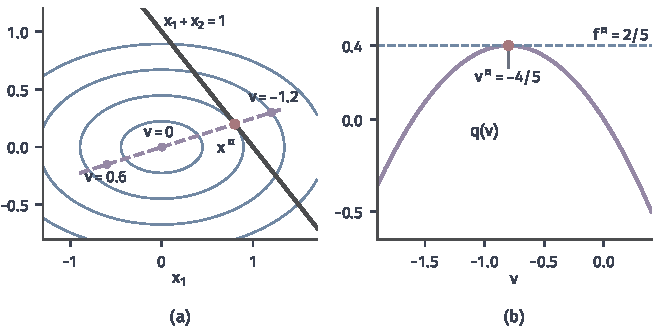
\includegraphics[width=112mm]{figures/05-optimization/06-constrained-optimization/matplotlib/dual-equality-q/figure.pdf}
 \caption{二次例~\eqref{eq:dual-quad}的对偶函数。(a)~蓝线是目标的等高线，深灰粗线是约束$x_1+x_2=1$，紫色虚线是内层最小点$\bm{x}(\nu)=(-\nu,-\nu/4)$的轨迹，红点是$\bm{x}^\star$。(b)~紫线是$q(\nu)$，它处处不超过蓝色虚线$f^\star$，在$\nu^\star=-4/5$处相等。}
 \label{fig:dual-equality-q}
\end{BookInlineFigure}

不等式约束的对偶函数要多处理一件事：内层的$\bm{D}$可以有边界，最小点会在边界上换挡。第~\ref{chap:constrained-optimality}章的预算例取$\tau=2$，就是这种情形，全章称它为\emph{预算例}：
\begin{equation}
 \min_{\bm{x}\geq\bm{0}}\ \frac12\bigl[(x_1-2)^2+(x_2-1)^2\bigr]\quad\text{s.t.}\quad x_1+x_2-2\leq0.
 \label{eq:dual-budget}
\end{equation}
把$\bm{x}\geq\bm{0}$留在$\bm{D}=\mathbb{R}^2_{+}$中，只给预算约束配乘子$\lambda\geq0$。

此时内层问题按坐标分开：
\[
 \min_{x_1\geq0}\Bigl[\frac12(x_1-2)^2+\lambda x_1\Bigr]+\min_{x_2\geq0}\Bigl[\frac12(x_2-1)^2+\lambda x_2\Bigr]-2\lambda.
\]
每一项是开口向上的一元二次函数在半轴上的最小化，最小点是无约束最小点截断到非负：
\[
 x_1(\lambda)=\max\{2-\lambda,0\},\qquad x_2(\lambda)=\max\{1-\lambda,0\}.
\]

$\lambda$越过$1$时第二个坐标碰到边界，越过$2$时第一个坐标也碰到边界。分三段代入，得到
\begin{equation}
 q(\lambda)=\begin{cases}
 \lambda-\lambda^2, & 0\leq\lambda\leq1,\\
 \dfrac12-\dfrac12\lambda^2, & 1\leq\lambda\leq2,\\
 \dfrac52-2\lambda, & \lambda\geq2.
 \end{cases}
 \label{eq:dual-budget-q}
\end{equation}

三段在分界点连续：$\lambda=1$时都是$0$，$\lambda=2$时都是$-3/2$。第一段的最大点是$\lambda^\star=1/2$，最好的下界是$q(1/2)=1/4$。

这个例子的解是$\bm{x}^\star=(3/2,1/2)$，目标值$\frac12(\frac14+\frac14)=\frac14$，下界再次与最优值相等。图~\ref{fig:dual-budget-q}中，内层最小点随$\lambda$增大沿折线向原点移动，价格越高，用得越少；$q$相应地分成三段。

\begin{BookInlineFigure}
 \centering
 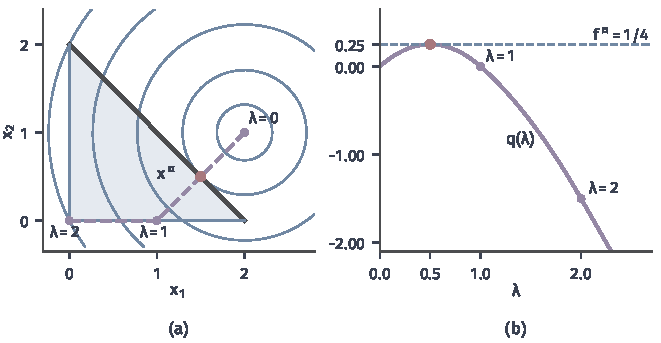
\includegraphics[width=112mm]{figures/05-optimization/06-constrained-optimization/matplotlib/dual-budget-q/figure.pdf}
 \caption{预算例~\eqref{eq:dual-budget}的对偶函数。(a)~浅蓝区域是可行集，深灰粗线是预算约束，蓝线是目标等高线，紫色虚线是内层最小点$\bm{x}(\lambda)$随$\lambda$从$0$增大的轨迹，紫点是$\lambda=0,1,2$时的位置，红点是$\bm{x}^\star$。(b)~紫线是分段的$q(\lambda)$，紫点是分界点，红点是最大点$(1/2,1/4)$。}
 \label{fig:dual-budget-q}
\end{BookInlineFigure}

\subsection{对偶问题}
\label{sec:dual-problem}

每组合法的乘子给出一个下界，下界越大提供的信息越多。很自然地，我们想要最大的那个，于是得到一个新的优化问题。

\begin{definition}[对偶问题]
 \label{def:dual-problem}
 问题~\eqref{eq:dual-primal}的对偶问题是在合法乘子上最大化对偶函数，
 \begin{equation}
  d^\star=\sup_{\bm{\lambda}\geq\bm{0},\ \bm{\nu}}q(\bm{\lambda},\bm{\nu}),
  \label{eq:dual-problem}
 \end{equation}
 其最优值$d^\star$可以取$\pm\infty$；对偶可行的乘子不存在时$d^\star=-\infty$。达到这个上确界的乘子称为对偶最优乘子。
\end{definition}

这里的约束只有$\bm{\lambda}\geq\bm{0}$，比原问题简单。更值得注意的是目标函数的形状。图~\ref{fig:dual-budget-q}(b)和图~\ref{fig:dual-equality-q}(b)中的$q$都是凹的，这不是巧合。

要看出原因，把$\mathcal{L}$反过来读：固定$\bm{x}$，它关于乘子是仿射函数，斜率是约束值$g_i(\bm{x})$与$h_j(\bm{x})$，截距是$f(\bm{x})$。$q$是这一族直线的下包络。图~\ref{fig:dual-affine-envelope}中一元例的每条直线对应一个$x$，它们的下包络（紫线）向下弯曲。

\begin{theorem}[对偶函数是凹的]
 \label{thm:dual-concave}
 对问题~\eqref{eq:dual-primal}，无论$f,g_i,h_j$和$\bm{D}$是否凸，$q$都是凹函数，$\operatorname{dom}q$是凸集。
\end{theorem}

\begin{proof}
 记$\bm{a}=(\bm{\lambda},\bm{\nu})$。任取$\bm{a}_1,\bm{a}_2$和$\theta\in[0,1]$，令$\bm{a}=\theta\bm{a}_1+(1-\theta)\bm{a}_2$。$\mathcal{L}$对乘子是仿射的，所以对每个$\bm{x}\in\bm{D}$，
 \[
  \mathcal{L}(\bm{x},\bm{a})=\theta\mathcal{L}(\bm{x},\bm{a}_1)+(1-\theta)\mathcal{L}(\bm{x},\bm{a}_2).
 \]
 由下确界的定义，右端不小于$\theta q(\bm{a}_1)+(1-\theta)q(\bm{a}_2)$。对$\bm{x}\in\bm{D}$取下确界，得到
 \[
  q(\bm{a})\geq\theta q(\bm{a}_1)+(1-\theta)q(\bm{a}_2).
 \]
 若$\bm{a}_1,\bm{a}_2\in\operatorname{dom}q$，右端有限，于是$\bm{a}\in\operatorname{dom}q$。
\end{proof}

\begin{BookInlineFigure}
 \centering
 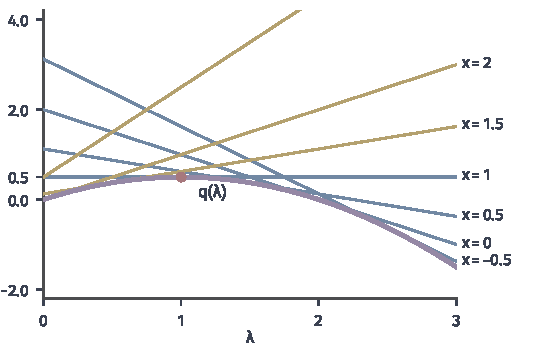
\includegraphics[width=92mm]{figures/05-optimization/06-constrained-optimization/matplotlib/dual-affine-envelope/figure.pdf}
 \caption{一元例中，每个固定的$x$给出一条直线$\lambda\mapsto\mathcal{L}(x,\lambda)$，蓝线对应可行的$x$，黄线对应不可行的$x$（最陡的一条是$x=3$），紫线是下包络$q(\lambda)=\lambda-\lambda^2/2$。可行点的直线斜率不为正，所以在$\lambda\geq0$上不超过其截距$f(x)$；水平粗线是$x=1$，高度为$f^\star=1/2$，在红点处与$q$相切。}
 \label{fig:dual-affine-envelope}
\end{BookInlineFigure}

定理~\ref{thm:dual-concave}说的是一个凸优化问题总摆在手边，无论原问题多么复杂，最大化一个凹函数原则上没有多余的局部最优。但这并不意味着对偶问题容易求解。计算$q$的一个值就要做一次内层的全局最小化，而内层目标$\mathcal{L}(\cdot,\bm{\lambda},\bm{\nu})$可以和原目标一样非凸。前面$f(x)=x^3-3x$的例子说明，局部解在这里给不出下界。凹性属于外层，难度可能全部留在内层。

线性规划是内层可以完全算出的特例。把第~\ref{chap:linear-programming}章的标准型$\min\bm{c}^\top\bm{x}$，$\bm{A}\bm{x}=\bm{b}$，$\bm{x}\geq\bm{0}$放进这个框架，取$\bm{D}=\mathbb{R}^n$。给不等式$-\bm{x}\leq\bm{0}$配乘子$\bm{s}\geq\bm{0}$，给等式配乘子$-\bm{y}$，则
\[
 \mathcal{L}=\bm{c}^\top\bm{x}-\bm{y}^\top(\bm{A}\bm{x}-\bm{b})-\bm{s}^\top\bm{x}=\bm{b}^\top\bm{y}+(\bm{c}-\bm{A}^\top\bm{y}-\bm{s})^\top\bm{x}.
\]

这是$\bm{x}$的线性函数，只有斜率为零时下确界才有限：
\[
 q(\bm{s},\bm{y})=\begin{cases}\bm{b}^\top\bm{y}, & \bm{A}^\top\bm{y}+\bm{s}=\bm{c},\\ -\infty, & \text{其他情形}.\end{cases}
\]
第~\ref{chap:linear-programming}章对偶问题的等式约束$\bm{A}^\top\bm{y}+\bm{s}=\bm{c}$，在这里的含义是$\operatorname{dom}q$的条件。把$q=-\infty$的乘子排除后，再最大化$\bm{b}^\top\bm{y}$，就回到了那里的对偶问题。
